

%%%%%%%%%%%%%%Empieza la presentacion%%%%%%%%%%%%%%%%%%%%%%%%%%%%%%%%%%%%

%\begin{frame}
%\frametitle{Esquema}
 %   \tableofcontents
%\end{frame}


\section{Cómputo eficiente}

%\subsection{Transformada Lineal}
%\subsection{Transformada Rápida de Fourier (FFT)}



%%%%%%%%%%%%%%%%%%%%%%%%%%%%%%

\begin{frame}
\frametitle{FFT: Cómputo eficiente de la DFT I}

\footnotesize

\hspace{3cm}\alert{$X(k)=\sum_{n=0}^{N-1} x(n) e^{-j\frac{2\pi}{N}kn}$}

\hspace{3cm}\alert{$x(n)=\frac{1}{N}\sum_{k=0}^{N-1} X(k) e^{j\frac{2\pi}{N}kn}$}

\begin{itemize}
\item Para calcular la DFT o la IDFT podemos construir (tal y como hicimos en el caso de la serie de Fourier discreta)  un sistema lineal en el que los coeficientes son los $e^{j\frac{2\pi}{N}kn}$.
\item Para simplificar las expresiones, definimos $W_N=e^{-j\frac{2\pi}{N}}$ y los coeficientes $e^{-j\frac{2\pi}{N}kn}=W_N^{kn}$. Se tiene que $X(k)=\sum_{n=0}^{N-1}x(n)W_N^{kn}$ con k=${0,1,\dots,N-1}$

{\scriptsize
$\left [\begin{array}{c}X(0)\\X(1)\\\vdots\\X(N-1)\end{array}\right ]=\left [\begin{array}{cccc}1& 1 &\dots &1\\ 1 &W_M^{1}& \dots& W_M^{N-1}\\\vdots&\vdots&\ddots & \vdots\\1 & W_M^{N-1} & \dots & W_M^{(N-1)(N-1)} \end{array}\right ]\left [\begin{array}{c}x(0)\\x(1)\\\vdots\\x(N-1)\end{array}\right ]$
}

\item Si la secuencia x(n) es muy larga, el computo a través del sistema lineal no es computacionalmente eficiente ($N^2$ sumas y $N^2$ multiplicaciones con complejos.

\item Existen algoritmos alternativos que permiten realizar la operación dividiendo las secuencias en secuencias más pequeñas. Estos algoritmos son lo que constituyen la \alert{FFT (Fast Fourier Transform)}.


\end{itemize}


\end{frame}

%%%%%%%%%%%%%%%%%%%%%%%%%


\begin{frame}
\frametitle{FFT: Cómputo eficiente de la DFT II}

\footnotesize


\color{olivegreen}{Ejemplo: Algoritmo en base 2 de diezmado temporal }{\scriptsize \color{gray} (hay algoritmos más rapidos)}


\begin{itemize}
\color{gray}
\item Suponemos que la longitud N es una potencia de 2 ($N=2^p$).
\item Dividir la secuencia x(n) en dos secuencias de longitud N/2, y agrupar los elementos con n impar y con n impar:

$X(k)=\sum_{n=0}^{N-1}x(n)W_N^{nk}=\sum_{n \in pares}  x(n)W_N^{nk} + \sum_{n \in impares}  x(n)W_N^{nk}=$

\hspace{0.8cm}$=\sum_{r=0}^{N/2-1} x(2r) W_N^{2rk}+\sum_{r=0}^{N/2-1} x(2r+1) W_N^{(2r+1)k}=$

\hspace{0.8cm}$=\sum_{r=0}^{N/2-1} f(r) W_{N/2}^{rk}+\sum_{r=0}^{N/2-1} g(r) W_N^k W_{N/2}^{r}=$

\hspace{0.8cm}$=F(k)+W_N^k G(k)$ para $k=\{0,...,N/2-1\}$

\item Necesitamos saber que les pasa a los puntos sucesivos. Como F(k) y G(k) son periódicas de periodo $N/2$, podemos calcular sus valores aprovechando dicha propiedad:

$X(k+N/2)=F(k)+W_N^{k+N/2} G(k)$ para $k=\{N/2,...,N-1\}$

\scriptsize
\item En la original teníamos $N^2$ sumas + $N^2$ productos. Aquí tenemos $(2*(N/2)^2$ sumas + $2*(N/2)^2$ productos + otros). La división de la secuencia en subsecuencias se puede repetir para  calcular $F(k)$ y $G(k)$.

\vspace{-0.2cm}


\rule{11cm}{0.4pt}

$f(r)=x(2r)$   y $g(r)=x(2r+1)$

F(k) y G(r) son las DFT de N/2 puntos de g(r) y h(r).


\end{itemize}
\end{frame}

\begin{frame}
\frametitle{Cómputo eficiente de la respuesta del sistema FIR}

\footnotesize

\begin{itemize}
\item Hemos visto que para calcular la respuesta de un sistema FIR podemos usar el producto de las DFTs.
\item Si la señal de entrada o la función ponderatriz son funciones de duración elevada, necesitaremos calcular sus DFTs de forma eficiente (FFT) y obtener el producto de las DFTs.
\item Alternativamente, siempre y cuando la longitud $L$ de secuencia de la señal de entrada $x(n)$ sea mucho mayor que la longitud $M$ de la función ponderatriz $h(n)$ se puede simplificar el calculo dividiendo la señal x(n) en subsecuencias de $L_D+M-1$ valores, con $L_D>>M$.

\item Existen diferentes formas de proceder (método de solapamiento y almacenamiento, o el método de solapamiento y adición) que agilizan el computo considerablemente.
\end{itemize}

\end{frame}


\begin{frame}
\frametitle{Cómputo eficiente  con Matlab I}

\footnotesize
\begin{itemize}

\item DFT:   \color{blue}{\textrm{X=fft(x)}}
\begin{itemize}
\footnotesize
\item \color{blue}{\textrm{x}} \color{black} es un vector con \color{blue}{\textrm{N=length(x)}} \color{black} elementos, y \color{blue}{\textrm{X}} \color{black} es su DFT con \color{blue}{\textrm{N}} \color{black}  elementos.
\item Si se quiere obtener una DFT con más elementos, rellenar con ceros al final de \color{blue}{\textrm{x}}\color{black}.
\item Como $X(k)=X(e^{j \frac{2\pi}{N}k})$, para representarlo frente a $\Omega$ discreta hacemos \color{blue}{\textrm{w=2*pi/N*[0:N-1]}}\color{black}. Además, al ser una Transformada de Fourier, es conveniente representar el modulo y el argumento por separado.

\item Si $x(n)$ es una señal muestreada de una señal continua $x_a(t)$ sin aliasing (i.e. que ha sido muestreada con un $T_s$ que adecuado), podemos representar el resultado de la fft  frente a $\omega$ continuo haciendo  \color{blue}{\textrm{w=2*pi/N*[0:N-1]/Ts}} \color{black}\color{black} ya que tal y como vimos en el tema de muestreo el espectro de la señal continua y la muestreada están relacionados por $X_d(e^{j\Omega})=\frac{1}{T_s}\!\! \sum_{k=-\infty}^{\infty}\!X_c(j(\frac{\Omega-2k\pi}{T_s}))$ .

\end{itemize}

\item \color{black}IDFT: \color{blue}{\textrm{x=ifft(X)}}

\end{itemize}

\end{frame}

%%%%%%%%%%%%%%%%%%%%%%%%%%%%%%%%%%%%%%%%


\begin{frame}
\frametitle{Cómputo eficiente  con Matlab II}

\footnotesize
\begin{itemize}

\item Respuesta del sistema:

\begin{itemize}
\footnotesize
\item  \color{blue}{\textrm{y=filter(num,den,x)}} \color{black} donde la función de transferencia del filtro $H(z)=\frac{num(z)}{den(z)}$.

\vspace{0.2cm}

\item Alternativamente, podemos llamar la orden anterior con la condiciones iniciales \color{blue}{\textrm{ci}} \color{black} previas: \color{blue}{\textrm{y=filter(num,den,x,ci)}} \color{black}. El valor de las condiciones iniciales se puede calcular con la orden \color{blue}{\textrm{ci=filtic(num,den,x0,y0)}} \color{black}, donde \color{blue}{\textrm{x0}} \color{black} e \color{blue}{\textrm{y0}} \color{black} son los valores de la entrada y salida en los instantes previos.

\vspace{0.2cm}

\item Si el filtro es FIR (den(z)=1) y las condiciones iniciales son nulas, la respuesta del sistema se puede calcular también con la orden \color{blue}{\textrm{y=conv(num,x)}}\color{black}.


\end{itemize}

\end{itemize}

\end{frame}

\begin{frame}
\frametitle{Ejemplo de cómputo de FFT I}

\footnotesize

\begin{columns}[c]
\begin{column}{7.5cm}

\color{olivegreen} Ejemplo: \color{black} Calcular las componentes en frecuencia de $N=500$ muestras de la $x_c(t)=sen(2\pi f_1 t)+sen(2\pi f_2 t)$ con $f_1=10; f_2=30; f_s=100$ con la FFT.

\vspace{-0.2cm}

\visible<2->{
  \lstinputlisting{./Respuestas/FFTMio.m}
}


\footnotesize
\color{gray}

\vspace{0.2cm}

\visible<6->{
Segun aumentamos $N$ la ventana es m\'{a}s grande y la $X(jw)$ se parece m\'{a}s a las de la $x_c(t)$. Adem\'{a}s tenemos m\'{a}s muestras de la DTFT $X(e^{jw})$
\color{black}}

\end{column}
\begin{column}{4cm}

\visible<3->{
\includegraphics[width=3cm]{./Figures/FFT1.eps}
}

\vspace{0.1cm}

\visible<4->{
\includegraphics[width=3cm]{./Figures/FFT2.eps}}

\vspace{0.1cm}

\visible<5->{
\includegraphics[width=3cm]{./Figures/FFT3.eps}}

\end{column}

\end{columns}



\end{frame}

%%%%%%%%%%%%%%%%%%%%%%%%%%%%%%%%%%%%%%%%


\begin{frame}
\frametitle{Ejemplo de cómputo de FFT II}

\footnotesize

\color{olivegreen} Ejemplo: \color{black} Continuaci\'{o}n.



\begin{columns}[c]
\hspace{0.5cm}\begin{column}{7.9cm}



Como $x_d(n)$ es real, el modulo de la FFT es par.

Como es peri\'{o}dica solo se representa entre $[0,N-1]$, $[0,2\pi]$ o $[0,Fs]$.

Ambas propiedades permiten cambiar la representaci\'{o}n al rango $[-N/2:N/2]$, $[-\pi,\pi]$, $[-Fs/2,Fs/2]$. Para trasladar la FFT hay que usar el comando \color{blue}{\textrm{X=fftshift(X)}}\color{black}.

\vspace{-0.4cm}

\lstinputlisting{./Respuestas/FFTMio2.m}






\end{column}
\hspace{0.1cm}\begin{column}{3.5cm}
\vspace{0.1cm}

FFT directa (frente $f_c$)

\vspace{0.1cm}

\includegraphics[width=3cm]{./Figures/FFT3.eps}

\vspace{0.2cm}

 FFT transladada (vs $f_c$)

\vspace{0.1cm}

\includegraphics[width=3cm]{./Figures/FFT6.eps}


\end{column}

\end{columns}


\end{frame}


\begin{frame}
\frametitle{Ejemplo de cómputo de FFT III}

Por lo general, nos dar\'{a}n ya la se\~{n}al discreta. Esta puede haber sido originada:

\small

\begin{itemize}
\item Directamente en discreto (porque ya nos den la expresi\'{o}n discreta o sea el resultado de un sistema discreto). \visible<2->{ En esos casos, podemos representarla respecto a $w_d$ o $f_d$. } \visible<3->{Pero debemos tener en cuenta que no representamos la DTFT si no unas muestras de la misma).}

\item \visible<4->{Muestreando una se\~{n}al continua (como hemos hecho en el ejemplo).} \visible<5->{En esos casos, conocemos el periodo de muestreo, por lo que podemos representarla frente a $w_c$ o $f_c$.}\visible<6->{Pero hay que tener en cuenta que a trav\'{e}s de la FFT estamos aproximando triplemente la CTFT (enventanar la se\~{n}al al generar un n\'{u}mero finito de muestras puede cambiar su espectro, el $T_s$ no debe producir aliasing y la FFT son muestras de la DTFT).}

\visible<7->{
\item El rango de las frecuencias utilizado (p.e. $[0, F_s]$ o $[-F_s/2, F_s/2]$) es indiferente, siempre y cuando la representaci\'{o}n este bien hecha  y se sepa interpretar la FFT. }

\end{itemize}


\end{frame}
